% arXiv builds through DVI unless told otherwise, and the DVI route cannot embed
% PNG. This paper loads orcid.png, so pdfLaTeX is required. arXiv reads this
% declaration only within the first five lines of the main file.
\pdfoutput=1

\documentclass{article}

\usepackage{arxiv}

\usepackage[utf8]{inputenc}
\usepackage[T1]{fontenc}
\usepackage{hyperref}
\usepackage{url}
\usepackage{booktabs}
\usepackage{amsmath}
\usepackage{amssymb}
\usepackage{microtype}
\usepackage{graphicx}
\usepackage{natbib}
\usepackage{doi}
\usepackage{xcolor}
\usepackage{tikz}
\usepackage{enumitem}

% Figure 1's two series. Okabe-Ito blue and vermillion, which stay
% distinguishable under the common colour vision deficiencies; the two
% series also differ in dash pattern and in marker, so the figure reads
% in greyscale with no colour at all.
\definecolor{knowInk}{HTML}{0072B2}
\definecolor{adoptInk}{HTML}{D55E00}

\hypersetup{
  colorlinks=true,
  linkcolor=blue!70!black,
  citecolor=green!50!black,
  urlcolor=blue!60!black,
  pdftitle={Probability Is Not an Answer: Rank-Level Measurement of Knowledge Conflict in Small Language Models},
  pdfsubject={cs.CL},
  pdfauthor={Amey Thakur, Sarvesh Talele},
  pdfkeywords={Knowledge Conflict, Retrieval-Augmented Generation, Language Models, Evaluation Methodology},
}

\title{Probability Is Not an Answer: Rank-Level Measurement of\\ Knowledge Conflict in Small Language Models}

\author{
	\href{https://orcid.org/0000-0001-5644-1575}{
\includegraphics[scale=0.06]{orcid.png}\hspace{1mm}Amey Thakur} \\
	Independent Researcher \\
	Toronto, Canada \\
	\texttt{ameythakur20@gmail.com} \\
	\And
	\href{https://orcid.org/0009-0002-0818-461X}{
\includegraphics[scale=0.06]{orcid.png}\hspace{1mm}Sarvesh Talele} \\
	Independent Researcher \\
	Mumbai, India \\
	\texttt{talelesarvesh@gmail.com} \\
}

\renewcommand{\undertitle}{}
\renewcommand{\headeright}{}
\renewcommand{\shorttitle}{Probability Is Not an Answer}

\date{October 15, 2026}

% Generated by experiments/make_paper_numbers.py. Do not edit.
\newcommand{\NRows}{864}
\newcommand{\NDoc}{432}
\newcommand{\NModels}{6}
\newcommand{\OverallUpdate}{61.6}
\newcommand{\OverallStale}{20.6}
\newcommand{\MedianPhrasingSpread}{47.9}
\newcommand{\ProbOverTen}{332}
\newcommand{\ProbOverTenNotTop}{69}
\newcommand{\ProbOverTenNotTopPct}{20.8}
\newcommand{\KnowsMin}{25.0}
\newcommand{\KnowsMax}{98.6}
\newcommand{\PerModel}{72}
\newcommand{\NConflict}{304}
\newcommand{\AdoptConflict}{66.8}
\newcommand{\KeepConflict}{27.3}
\newcommand{\AdoptMin}{38.6}
\newcommand{\AdoptMax}{91.8}
\newcommand{\AdoptQwenSmall}{91.8}
\newcommand{\AdoptQwenLarge}{87.3}
\newcommand{\AdoptTiny}{38.6}
\newcommand{\KeepTiny}{57.1}
\newcommand{\KnowsTiny}{97.2}
\newcommand{\KeepQwenLarge}{0.0}
\newcommand{\NConflictTiny}{70}
\newcommand{\MaxPhrasingSpread}{87.5}
\newcommand{\QwenSmallBest}{100.0}
\newcommand{\QwenSmallWorst}{12.5}
\newcommand{\MedianAdoptSpread}{35.1}
\newcommand{\MaxAdoptSpread}{57.6}
\newcommand{\NAdoptSpread}{4}
\newcommand{\QwenSmallConflictsWorst}{1}
\newcommand{\QwenSmallAdoptSpread}{16.7}
\newcommand{\TinyAdoptLow}{17.4}
\newcommand{\TinyAdoptHigh}{75.0}


\begin{document}
\maketitle

\begin{abstract}
A retrieval-augmented system succeeds only when the document it supplies beats
what the model already believes. We measure which one wins, at the level of the
token the model would actually emit, over \NRows\ forward passes: \NModels\ open
models from 124M to 1.5B parameters, 24 counterfactual probes, three phrasings,
with and without a contradicting document. Restricting to the \NConflict\ cases
where the model demonstrably held the fact beforehand, the document is adopted
\AdoptConflict\% of the time and the model keeps its own answer \KeepConflict\%.
Which model defers is not predicted by size. Holding the fact rises
monotonically with parameter count, from \KnowsMin\% to \KnowsMax\%, but
adoption does not: TinyLlama-1.1B holds the fact \KnowsTiny\% of the time and
still adopts the document least of the six, at \AdoptTiny\%, while
Qwen2.5-0.5B, a third its size, adopts \AdoptQwenSmall\%. Wording moves the
result nearly as much as the model does: over all probes the rate spreads by a
median of \MedianPhrasingSpread\ percentage points across three paraphrases, and
restricted to conflicts, where the spread measures deference rather than
recall, it still reaches \MaxAdoptSpread. We also show why
this has to be read at the rank: the in-context answer carries more than $0.10$
of the probability mass in \ProbOverTen\ conditions and is still not what the
model says in \ProbOverTenNotTop\ of them, \ProbOverTenNotTopPct\%. That gap is
not hypothetical. It is how an earlier version of this work reached a published
conclusion that the measurement did not support, which we correct here. All
code, probes and measurements are public.
\end{abstract}

% ============================================================
\section{Introduction}
% ============================================================

A retrieval-augmented system puts a document in front of a language model and
expects the model to use it. When the document contradicts what the model
learned in training, one of the two has to give, and which one gives is the
question this paper measures. It is not hypothetical: a clinical assistant
reading a withdrawal notice, or a coding assistant reading a deprecation note,
is useful only if the document wins.

The measurement is easy to get wrong, and we got it wrong. An earlier version of
this work concluded that models resist a corrective document, on the strength of
the probability the model assigned to the expected answer. That quantity can be
small while the model would nonetheless answer correctly, because the mass is
spread over a vocabulary of tens of thousands of tokens and the expected answer
needs only to be ranked first, not to be large. Re-running the same probes with
the rank recorded showed the conclusion did not hold
(Section~\ref{sec:correction}). This paper reports the measurement done
properly, and the size of the gap we fell into is itself one of the results.

Two changes make it proper. First, we record what the model would actually say,
the top-ranked continuation, alongside the probability. Second, we use
counterfactual probes rather than real-world updates. A real-world update
creates a conflict only for a model whose training data predates it, so across
models of different vintages the conflict is present for some and absent for
others, and a probability-only readout cannot tell those two cases apart. A
counterfactual document asserts something every model is confident is false, so
the conflict is present by construction for all of them. This is the standard
device in the knowledge-conflict
literature~\citep{longpre2021entity, xie2024conflicts}.

Our contributions are:

\begin{enumerate}[leftmargin=*]
  \item A rank-level measurement of parametric--context conflict over \NRows\
    forward passes, reported on the \NConflict\ probe-phrasing pairs where the
    model demonstrably held the fact and a conflict therefore existed.
  \item The finding that deference to a document is not a function of scale.
    Holding the fact rises monotonically with parameter count across the six
    models; adopting the document does not, and the 1.1B model that holds the
    fact most reliably defers least.
  \item Evidence that the question's wording moves the outcome nearly as much
    as the choice of model, by up to \MaxAdoptSpread\ percentage points of
    deference alone, and a separation of that effect from the larger one the
    wording has on whether the model holds the fact at all
    (Section~\ref{sec:phrasing}).
  \item Evidence that a probability-only readout cannot support a claim about
    what a model answers, and a correction of our own earlier report on exactly
    that ground (Section~\ref{sec:correction}).
\end{enumerate}

Code, probe set and measurements are public~\citep{thakur2026code}.

% ============================================================
\section{Method}
\label{sec:method}
% ============================================================

\paragraph{Probes.} Each probe is a country whose capital no model of this size
should get wrong, paired with a counterfactual that is a real, prominent city of
the same country: France and Lyon, Japan and Osaka, Egypt and Alexandria, and 21
others. Using a real city keeps the substitution plausible rather than
nonsensical. Holding the fact type fixed across all 24 probes means that a
difference between probes is not a difference between kinds of question. The
document asserts the substitution as a constitutional relocation and names the
new capital twice.

\paragraph{Phrasings.} Each probe is asked three ways, differing in wording but
not in what is asked. A quantity that moves across the three is a property of the
sentence rather than of the model's knowledge, and reporting the spread is what
lets a reader tell those apart.

\paragraph{Conditions.} Every probe and phrasing is run twice: once with the
question alone, which measures what the model believes, and once with the
contradicting document prepended, which measures what it does about the
conflict. The first condition is not a control in name only. It is what
identifies the subset in which a conflict exists at all, and every headline
number in this paper is restricted to that subset.

\paragraph{Models.} Six open models spanning an order of magnitude: GPT-2 at
124M, 355M and 774M~\citep{radford2019language}, Qwen2.5-0.5B-Instruct and
Qwen2.5-1.5B-Instruct~\citep{yang2024qwen2}, and
TinyLlama-1.1B-Chat~\citep{zhang2024tinyllama}. All run in float32 on CPU, so the
numbers reproduce on ordinary hardware rather than depending on a particular
accelerator's arithmetic.

\paragraph{What is recorded.} For a prompt $x$ the model defines a distribution
$p_\theta(\cdot \mid x)$ over the vocabulary. Writing $t$ for the first token of
the true answer and $c$ for the first token of the counterfactual, we record
$p_\theta(t \mid x)$ and $p_\theta(c \mid x)$, the rank of each, and
$\arg\max_v p_\theta(v \mid x)$. Rank determines the answer under greedy
decoding; probability is what the earlier report used alone.

That distribution is the softmax over the final layer's output, the standard
construction for a transformer decoder~\citep{vaswani2017attention}, and we
follow the usual account of the feed-forward blocks and the softmax that turns
their output into a distribution~\citep{thakur2021fundamentals}. One consequence
of training by maximum likelihood matters here: such a model spreads mass over
everything the context makes plausible rather than committing to a single
continuation, unlike a generator trained against a
discriminator~\citep{thakur2021gan}. That is precisely why a modest probability
does not mean the token is not the answer, and it is the mechanism behind the
gap reported in Section~\ref{sec:rank}.

Answers are compared at the first token. Tokeniser boundaries were checked for
every probe, phrasing and model: all 144 country--answer pairs tokenise cleanly
across the three tokeniser families used here, so no probe silently measures a
merged token.

% ============================================================
\section{Results}
% ============================================================

Table~\ref{tab:results} reports all six models, and Figure~\ref{fig:scale} draws
the two columns the paper turns on.

\begin{table}[t]
\centering
\begin{tabular}{lrrrrrr}
\toprule
& Params & Knows & & Adopts & Keeps & Phrasing \\
Model & (M) & the fact & $n$ & the document & its own & spread \\
\midrule
GPT-2 & 124 & 25.0\% & 18 & 50.0\% & 16.7\% & 62.5 \\
GPT-2 medium & 355 & 54.2\% & 39 & 43.6\% & 56.4\% & 41.7 \\
GPT-2 large & 774 & 79.2\% & 57 & 75.4\% & 24.6\% & 29.2 \\
Qwen2.5-0.5B-Instruct & 494 & 68.1\% & 49 & 91.8\% & 8.2\% & 87.5 \\
TinyLlama-1.1B-Chat & 1100 & 97.2\% & 70 & 38.6\% & 57.1\% & 54.2 \\
Qwen2.5-1.5B-Instruct & 1540 & 98.6\% & 71 & 87.3\% & 0.0\% & 37.5 \\
\bottomrule
\end{tabular}
\caption{What each model does when a document contradicts it. \emph{Knows the fact} is how often the true capital is the top-ranked continuation with no document present, over \PerModel\ probe-phrasing pairs. The remaining columns are restricted to the $n$ pairs where that held, which are the cases in which a conflict actually exists: \emph{adopts the document} and \emph{keeps its own} are how often the counterfactual and the true answer respectively are top-ranked once the document is supplied. They need not sum to 100, because a model may rank a third token first. \emph{Phrasing spread} is the range, across the three wordings, of the rate at which the counterfactual is top-ranked over all 24 probes of that wording, in percentage points; it is not restricted to conflicts, and Section~\ref{sec:phrasing} separates the two. Knowing the fact rises monotonically with parameter count; adopting the document does not.}
\label{tab:results}
\end{table}


% Generated by experiments/make_paper_numbers.py. Do not edit.
\begin{figure}[t]
\centering
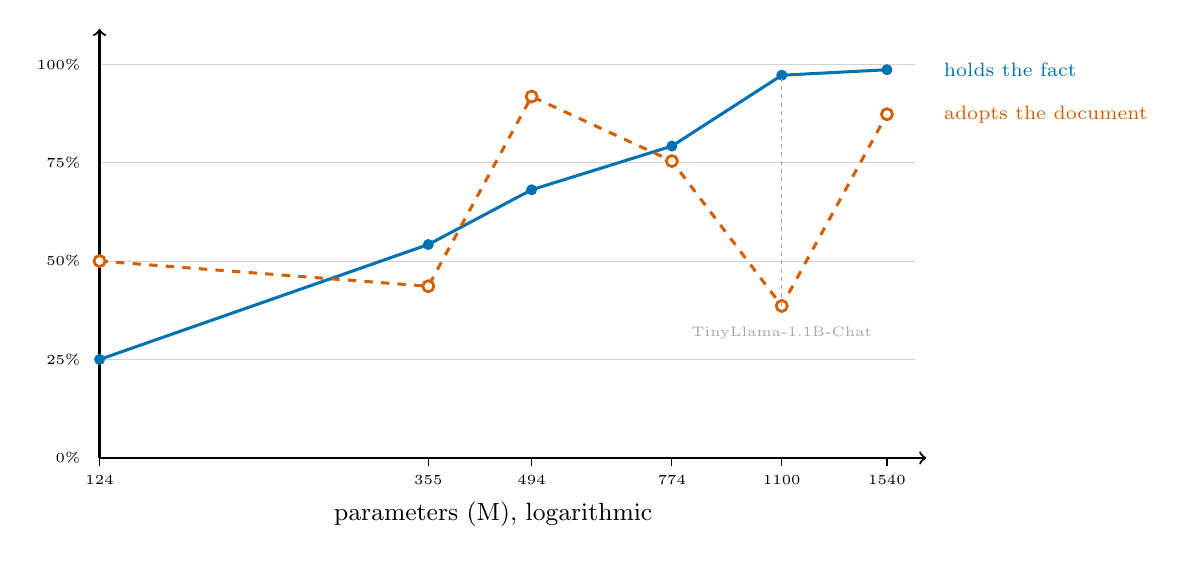
\begin{tikzpicture}[x=1cm, y=1cm]
  \draw[gray!35] (0,0.0) -- (10.35,0.0);
  \node[font=\tiny, anchor=east] at (-0.12,0.0) {0\%};
  \draw[gray!35] (0,1.25) -- (10.35,1.25);
  \node[font=\tiny, anchor=east] at (-0.12,1.25) {25\%};
  \draw[gray!35] (0,2.5) -- (10.35,2.5);
  \node[font=\tiny, anchor=east] at (-0.12,2.5) {50\%};
  \draw[gray!35] (0,3.75) -- (10.35,3.75);
  \node[font=\tiny, anchor=east] at (-0.12,3.75) {75\%};
  \draw[gray!35] (0,5.0) -- (10.35,5.0);
  \node[font=\tiny, anchor=east] at (-0.12,5.0) {100\%};
  \draw[->, thick] (0,0) -- (10.5,0);
  \draw[->, thick] (0,0) -- (0,5.45);
  \draw (0.0,0) -- (0.0,-0.1) node[below, font=\tiny] {124};
  \draw (4.175,0) -- (4.175,-0.1) node[below, font=\tiny] {355};
  \draw (5.487,0) -- (5.487,-0.1) node[below, font=\tiny] {494};
  \draw (7.269,0) -- (7.269,-0.1) node[below, font=\tiny] {774};
  \draw (8.664,0) -- (8.664,-0.1) node[below, font=\tiny] {1100};
  \draw (10.0,0) -- (10.0,-0.1) node[below, font=\tiny] {1540};
  \node[font=\small] at (5,-0.72) {parameters (M), logarithmic};
  \draw[line width=1.1pt, knowInk] (0.0,1.25) -- (4.175,2.71) -- (5.487,3.405) -- (7.269,3.96) -- (8.664,4.86) -- (10.0,4.93);
  \fill[knowInk] (0.0,1.25) circle (2pt);
  \fill[knowInk] (4.175,2.71) circle (2pt);
  \fill[knowInk] (5.487,3.405) circle (2pt);
  \fill[knowInk] (7.269,3.96) circle (2pt);
  \fill[knowInk] (8.664,4.86) circle (2pt);
  \fill[knowInk] (10.0,4.93) circle (2pt);
  \node[font=\scriptsize, anchor=west, knowInk] at (10.6,4.93) {holds the fact};
  \draw[line width=1.1pt, adoptInk, dashed] (0.0,2.5) -- (4.175,2.18) -- (5.487,4.59) -- (7.269,3.77) -- (8.664,1.93) -- (10.0,4.365);
  \draw[adoptInk, fill=white, line width=1pt] (0.0,2.5) circle (2pt);
  \draw[adoptInk, fill=white, line width=1pt] (4.175,2.18) circle (2pt);
  \draw[adoptInk, fill=white, line width=1pt] (5.487,4.59) circle (2pt);
  \draw[adoptInk, fill=white, line width=1pt] (7.269,3.77) circle (2pt);
  \draw[adoptInk, fill=white, line width=1pt] (8.664,1.93) circle (2pt);
  \draw[adoptInk, fill=white, line width=1pt] (10.0,4.365) circle (2pt);
  \node[font=\scriptsize, anchor=west, adoptInk] at (10.6,4.365) {adopts the document};
  \draw[gray!70, dash pattern=on 1.5pt off 1.5pt] (8.664,1.93) -- (8.664,4.86);
  \node[font=\tiny, gray!70, anchor=north] at (8.664,1.79) {TinyLlama-1.1B-Chat};
\end{tikzpicture}
\caption{Holding a fact scales with parameter count; deferring to a document that contradicts it does not. Filled markers are how often the model ranks the true answer first with no document present; open markers are how often it ranks the document's answer first, over the conflicts only, so the second curve is conditioned on the first. The first is monotone in size with no inversion anywhere; the second is not ordered by size at all. The dashed segment marks TinyLlama-1.1B, which holds the fact second most reliably of the six and defers least. Coordinates are generated from the same measurement as Table~\ref{tab:results}.}
\label{fig:scale}
\end{figure}


\subsection{Holding a fact scales; deferring to a document does not}

Whether a model holds the fact at all rises monotonically with parameter count,
from \KnowsMin\% at 124M to \KnowsMax\% at 1.5B, with no inversion anywhere in
the ordering. This is the expected result and serves mainly as a check that the
probes measure what they are meant to.

What the model then does with a contradicting document follows no such pattern.
Across the \NConflict\ genuine conflicts the document is adopted
\AdoptConflict\% of the time and the model keeps its own answer \KeepConflict\%,
but the per-model rates run from \AdoptMin\% to \AdoptMax\% in an order that has
little to do with size. The clearest case is TinyLlama-1.1B: it holds the fact
\KnowsTiny\% of the time, the second-highest of the six, and yet adopts the
document in only \AdoptTiny\% of its \NConflictTiny\ conflicts, keeping its own
answer in \KeepTiny\%. Qwen2.5-0.5B, less than half its size, adopts
\AdoptQwenSmall\%. The two Qwen models, at 494M and 1540M, are the two most
deferential; the three GPT-2 models and TinyLlama are not ordered by size among
themselves.

The natural reading is that deference is a property of how a model was trained
rather than of how large it is. We cannot separate those factors here: the six
models differ in family, in instruction tuning and in scale at once, and the
design does not let us hold two fixed while varying the third. What the data do
establish is the negative claim, which is the one that matters for practice:
scale alone does not buy a model that uses the document in front of it.
Qwen2.5-1.5B is the only model in the set that never keeps its own answer once
contradicted, at \KeepQwenLarge\%.

\subsection{Wording moves the answer, and moves two things at once}
\label{sec:phrasing}

How the question is worded changes the outcome substantially, and separating
what it changes is worth doing, because the two mechanisms carry different
advice.

The coarse quantity is the rate at which the counterfactual is top-ranked over
all 24 probes of a wording, with no restriction to conflicts. Across the three
wordings it has a median spread of \MedianPhrasingSpread\ percentage points and
a maximum of \MaxPhrasingSpread, and that maximum is Qwen2.5-0.5B, which ranks
the counterfactual first \QwenSmallBest\% of the time under its most favourable
wording and \QwenSmallWorst\% under its least.

That figure is not a measure of deference, and reading it as one is a mistake of
the same shape as the one Section~\ref{sec:correction} corrects. Under its third
wording Qwen2.5-0.5B holds the fact in \QwenSmallConflictsWorst\ of its 24
probes rather than in all 24, so there is almost no conflict left
for it to resolve; in the single conflict that remains it does adopt the
document. Restricted to conflicts, its adoption rate across the three wordings
is \QwenSmallAdoptSpread\ points wide, not \MaxPhrasingSpread. Most of what the
wording moved was whether the model knew the fact, not whether it deferred.

Deference does move, and by less. The adoption spread is defined only for the
\NAdoptSpread\ models whose every wording leaves at least one conflict, and over
those it has a median of \MedianAdoptSpread\ percentage points and a maximum of
\MaxAdoptSpread. The maximum is TinyLlama-1.1B, which adopts the document
\TinyAdoptLow\% of the time under one wording and \TinyAdoptHigh\% under
another, on conflicts in every case.

Either way the practical conclusion stands, and the second version states it
more precisely: a spread of \MaxAdoptSpread\ points in deference alone is larger
than the gap between most pairs of models in Table~\ref{tab:results}. A
single-phrasing result about knowledge conflict, including any single-phrasing
result in the earlier version of this work, reports a property of the sentence
at least as much as a property of the model. It also has to say which rate it is
reporting, since the two differ here by a factor of five on the same model.

\subsection{Probability is not an answer}
\label{sec:rank}

The in-context answer carries more than $0.10$ of the probability mass in
\ProbOverTen\ of the \NDoc\ conditions with the document present, and in
\ProbOverTenNotTop\ of those, \ProbOverTenNotTopPct\%, it is still not the token
the model ranks first. A reader given only the probability would conclude the
document had landed; a reader given the rank would see that the model would say
something else.

The converse also holds and is the trap we fell into. A small probability for the
expected answer is compatible with that answer being ranked first, because the
mass is distributed over a large vocabulary. Neither direction of inference from
probability to answer is safe. Recording the rank costs one comparison against
the maximum, and it is the only quantity that corresponds to what a system
deployed under greedy decoding will actually produce.

% ============================================================
\section{A correction to our earlier report}
\label{sec:correction}
% ============================================================

An earlier version of this work reported that across six models and three
documented fact changes the conflict did not resolve, and that no model answered
a drug-withdrawal probe correctly under any of three phrasings. That claim was
wrong, and the manner of its wrongness is the reason this paper exists.

The script that produced it recorded, for each model and phrasing, the surprisal
of the expected answer with the document present. It recorded neither the rank of
that answer nor the identity of the top-ranked token. A claim about what a model
answers cannot be derived from that quantity, and when we re-ran the same probes
with the rank recorded, three of the six models ranked the corrected answer first
under two of the three phrasings.

A second defect was structural. The probes were real-world updates, so whether a
model held the superseded fact depended on its training cutoff, and the six
cutoffs differ. For the drug probe the event predates every model's training
data, so no model held the superseded fact and there was no conflict to resist.
The large surprisal we reported was the question frame declining a participle,
not a model defending a stale belief. Both defects are removed by the design in
Section~\ref{sec:method}: counterfactual probes make the conflict independent of
cutoff, and the no-document condition identifies the cases where the model
actually held the fact.

We report this at length because the correction generalises. A probability-only
readout is cheap to compute and easy to tabulate, and it will return a number for
any probe whether or not that probe tests anything at all. Both defects would
have been caught immediately by recording the rank, which is one comparison.

% ============================================================
\section{Related work}
% ============================================================

\paragraph{What the readout should be.}
Factual probing of language models has used the top-ranked continuation as
its readout since \citet{petroni2019lama} posed the question, and the
quantity reported there is accuracy at rank one rather than a probability.
This paper's methodological claim is therefore not a new proposal but a
return to the existing convention, and the correction in
Section~\ref{sec:correction} is a case of having departed from it. The
reason the convention is the right one is that probability mass and rank
come apart: the mass is divided over tens of thousands of tokens and over
the several surface forms of one answer, so a small probability is
compatible with rank one and a large one with rank two.
\citet{min2022rethinking} make the general form of the point for in-context
learning, where the quantity a prompt moves is not the quantity the model
acts on. Section~\ref{sec:rank} measures how often the two disagree here:
in \ProbOverTenNotTopPct\% of the conditions where the document's answer
carries more than $0.10$ of the mass, it is still not what the model would
say.

\paragraph{What the wording does.}
That a paraphrase of a probe changes what a model appears to know is
established. \citet{jiang2020know} show that the prompt used to query a
model changes how much knowledge is extracted from it, and build a prompt
archive precisely because no single phrasing is representative.
\citet{elazar2021consistency} measure consistency directly over 328
paraphrases of 38 relations and find pretrained models frequently
inconsistent under paraphrase, which is the effect Section~\ref{sec:phrasing}
observes. Our contribution there is narrower and, we think, the part that
matters for a retrieval system: the wording moves two things at once, whether
the model holds the fact and whether it defers once it does, and the first
effect is much the larger. Reporting only their sum, as the first version of
this measurement did, attributes to deference a swing that mostly belongs to
recall.

\paragraph{What scale is expected to buy.}
The expectation that a capability improves with parameter count is the
default reading of the scaling literature~\citep{kaplan2020scaling,
hoffmann2022chinchilla}, and it holds here for one of the two quantities we
measure: whether the model holds the fact at all rises monotonically across
the six models. It does not hold for the other. The natural alternative
explanation, which our design cannot isolate, is that deference is set by
post-training rather than by size: instruction tuning optimises a model to
follow what it is given~\citep{ouyang2022instructgpt, wei2022flan}, and the
two most deferential models in Table~\ref{tab:results} are the two
instruction-tuned ones. We state this as the hypothesis it is; separating
family, tuning and scale needs a design that holds two of the three fixed.

\paragraph{Whether a model uses the context it is given.}
That supplying a document does not guarantee the model uses it is itself a
measured phenomenon. \citet{liu2024lost} show that retrieved evidence is used
unevenly depending on where it sits in the context, and
\citet{chen2024benchmarking} score a retrieval-augmented system on four
abilities, one of which is what it does when the passage it is handed is
counterfactual. Both treat use of the
context as something to be verified rather than assumed, which is the
position this paper takes and the reason it conditions on a conflict
existing.

\paragraph{Knowledge conflict.}
Conflict between parametric memory and supplied context has been studied
directly. \citet{longpre2021entity} construct conflicts by substituting entities
in the retrieved passage, the device used here, and find models often prefer
their parametric answer. \citet{xie2024conflicts} elicit a model's parametric
belief first and then present conflicting evidence, reporting that receptiveness
depends on how coherent that evidence is; our finding that deference is not
ordered by scale is consistent with their account of receptiveness as a trained
disposition. \citet{du2024context} give a persuasion-score formulation
quantifying how far a context moves a model's answer distribution, which is a
distributional relative of the rank-level quantity we report, and
\citet{xu2024conflicts} survey the area.

The conflict matters because retrieval is standard
practice~\citep{lewis2020rag, guu2020realm, gao2023ragsurvey}, and because
editing the parametric memory directly~\citep{meng2022rome, meng2023memit} does
not remove the possibility that weights and context disagree at inference.
Non-parametric memory also requires an index over the embedding space, the role
played classically by hierarchical spatial
partitions~\citep{thakur2022quadtree}.

The six models measured here are the GPT-2 family~\citep{radford2019gpt2},
TinyLlama~\citep{zhang2024tinyllama} and two Qwen2.5
checkpoints~\citep{yang2024qwen2}; the mechanism by which a transformer
stores the facts they are probed for is described
by~\citet{geva2021kv}.

Framing the failure as a synchronisation problem is deliberate. Parametric memory
and retrieved context are two replicas of one fact, and the failure is that they
disagree with no protocol to settle which is current, the question a distributed
system answers with a synchronisation protocol~\citep{thakur2022clock}. A natural
response is to gate a representation on an auxiliary scalar carrying recency or
provenance, a construction with a long lineage in systems combining a learned
representation with an explicit membership or confidence
signal~\citep{thakur2021neurofuzzy}. We do not evaluate such a gate here; an
earlier version of this work proposed one, and we have removed it because nothing
in our measurements tests it.

% ============================================================
\section{Limitations}
% ============================================================

The models are small. The largest is 1.5B parameters, and behaviour at 7B and
above may differ. The non-monotonicity we report is evidence about this range.

The design confounds family, instruction tuning and scale. We can show that
adoption is not ordered by parameter count, which is a negative claim and is
supported, but we cannot attribute the variation to any one factor.

The probes are homogeneous by construction. Every one is a national capital,
which controls for question type at the cost of telling us nothing about numeric,
temporal or causal facts.

Counterfactual probes buy freedom from the cutoff confound at a price: the
document asserts something false, and a model trained to resist false premises
may refuse it for reasons unrelated to the recency of its knowledge. A deployed
retrieval system meets the opposite case, where the document is true and the
parametric memory is stale. The two share a mechanism but are not identical, and
a model that looks admirably deferential here may be deferential to
misinformation as well.

Answers are compared at the first token, sufficient here because the candidate
cities differ there, but not general. The measurement is of a single-turn
next-token distribution under greedy reading; systems that sample, reason over
several steps, or are prompted to weigh sources explicitly may behave
differently.

% ============================================================
\section{Conclusion}
% ============================================================

Across \NConflict\ genuine conflicts in \NModels\ open models, a contradicting
document is adopted \AdoptConflict\% of the time. Whether a given model adopts it
is not predicted by size: holding the fact rises monotonically with parameter
count while deference does not, and the model that holds facts second-most
reliably defers least of all. The wording of the question moves the rate by up to
\MaxPhrasingSpread\ percentage points, comparable to the spread between models.

The methodological result is the one we would most like carried forward. The
probability a model assigns to an answer and the answer it gives are different
quantities, they disagree in \ProbOverTenNotTopPct\% of the conditions measured
here, and a published conclusion of ours rested on the difference. Rank is one
comparison more expensive and is what a deployed system actually emits.

\paragraph{Future work.} The natural extension is multimodal. When the
contradicting evidence is an image rather than a passage the same question
arises with no token rank to read the answer from, and the systems where this
matters, image translation~\citep{thakur2021whitebox, thakur2021aoda} and
zero-shot visual detection~\citep{thakur2026accident}, where a model must lean on
parametric knowledge because no corrective document exists, are exactly those for
which the diagnostic is missing. A second direction is deployment: the
accompanying demonstration runs a model in the
browser~\citep{thakur2026demo}, the same client-side setting as other real-time
in-browser inference work~\citep{thakur2026gesture}, and a conflict diagnostic
cheap enough to run there would put the measurement where the retrieval happens.

\section*{Artefacts}

Code, probe set and measurements are at~\citep{thakur2026code}; the cross-model
sweep is also published as a notebook~\citep{thakur2026notebook}, and an
interactive demonstration runs in the browser~\citep{thakur2026demo}.

\bibliographystyle{unsrtnat}
\bibliography{references}

\end{document}
